%
% Chapter — Deployment
%
\chapter{Deployment} \label{cap:deployment}

This chapter describes how the components introduced in the previous chapters are
packaged, provisioned, and run in production. Whereas Chapter~\ref{cap:architecture}
presented the \emph{logical} architecture --- how the source code is organised into
modules and layers --- this chapter presents the \emph{physical} deployment view: the
container images, the services that run on the host, the reverse-proxy layers, and the
path an external request travels to reach the application. The two views are
complementary: the Spring Boot backend that appears as a single logical component in
Chapter~\ref{cap:architecture} is, at deployment time, one container image among
several orchestrated together.

The platform runs on a single virtual machine (VM). Almost every runtime component
runs as a Docker container, orchestrated through Docker Compose; the only exception is
the outermost reverse proxy, a system-level Nginx provisioned directly on the host to
terminate HTTPS. Figure~\ref{fig:deployment} shows the complete topology.

\begin{figure}[H]
      \begin{center}
            \resizebox{\textwidth}{!}{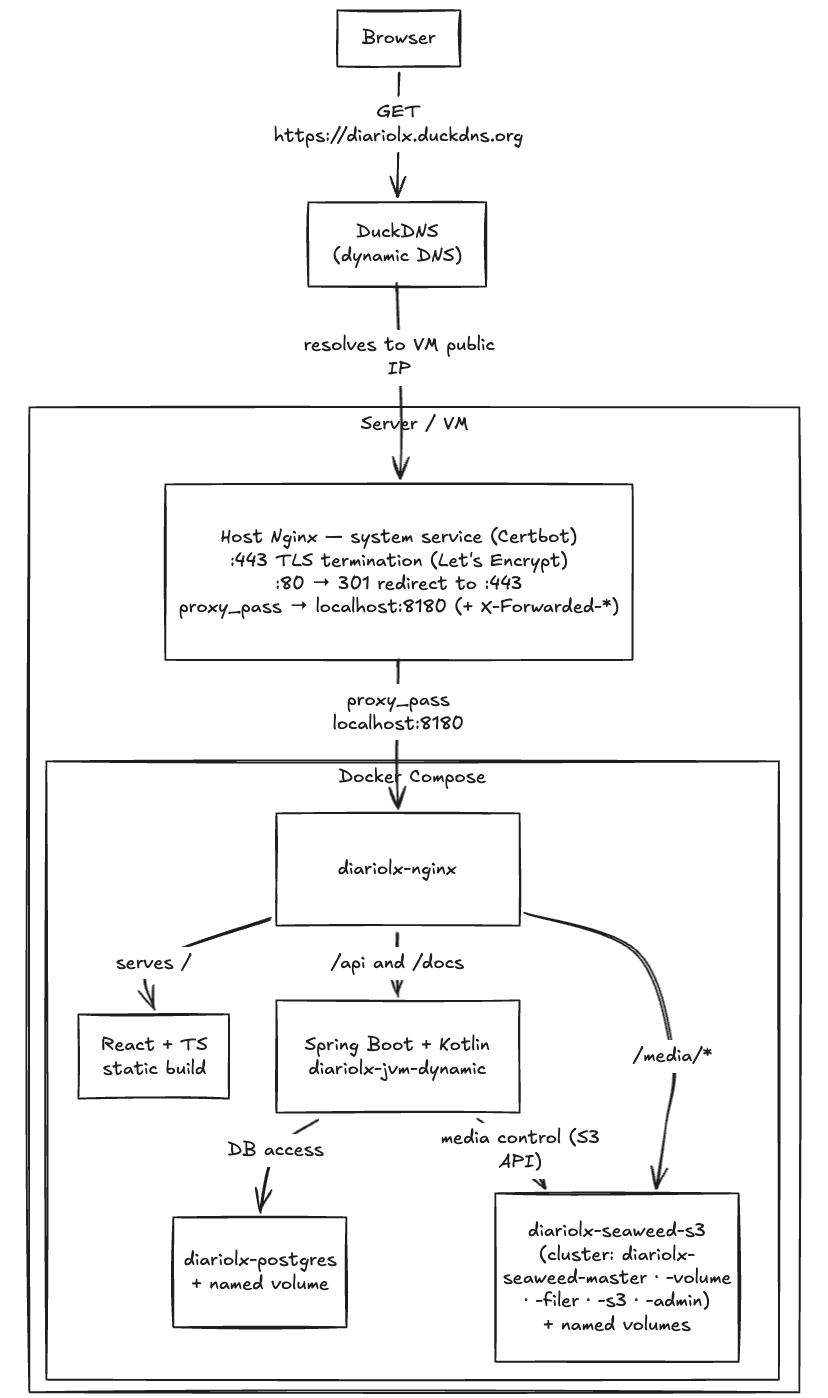
\includegraphics{./figures/deployment_diagram.png}}
      \end{center}
      \caption{Deployment topology of the \textit{Diário LX} platform.}
      \label{fig:deployment}
\end{figure}

\section{Container Images} \label{sec:dep_images}

The deployable images are built through a single Gradle aggregate task
(\texttt{buildImageAll}), which produces four images:

\begin{description}
      \item[\texttt{diariolx-jvm}] Built from \texttt{eclipse-temurin:21}. The Spring
            Boot application is split into three Docker layers --- external libraries,
            \texttt{META-INF} metadata, and the application classes --- so that the
            least-frequently-changed files occupy the lower, cacheable layers and only
            the application layer is rebuilt on most changes. The entry point launches
            \texttt{pt.ipl.diariolx.DiarioLXApplicationKt}.

      \item[\texttt{diariolx-nginx}] A multi-stage image that bundles \emph{both} the
            frontend and the reverse proxy. The first stage (\texttt{node:22-alpine})
            installs the frontend dependencies with \texttt{npm ci} and produces the
            React production build (\texttt{npm run build}) in \texttt{/app/dist}. The
            second stage (\texttt{nginx:alpine}) copies the Nginx configuration and the
            compiled build into the web root (\texttt{/usr/share/nginx/html}). Because
            the build context is the repository root, a single image has access to both
            the frontend sources and the shared Nginx configuration.

      \item[\texttt{diariolx-postgres}] A PostgreSQL image pre-provisioned with the
            database schema and seed data described in Chapter~\ref{cap:datamodel}.

      \item[SeaweedFS] The official \texttt{chrislusf/seaweedfs} image, used unchanged
            for the object-storage cluster.
\end{description}

\section{Orchestrated Services} \label{sec:dep_services}

Docker Compose orchestrates the following services on the VM:

\begin{itemize}
      \item \textbf{PostgreSQL} --- the relational database; its data is kept on a named
            volume so it survives container recreation, and its configuration is read
            from \texttt{.env.staging}.

      \item \textbf{SeaweedFS cluster} --- the self-hosted, S3-compatible object storage
            for multimedia assets, split into cooperating roles: a \emph{master}
            (cluster coordination), a \emph{volume} server (stores the file bytes), a
            \emph{filer} (filesystem semantics over the volumes), an \emph{S3 gateway}
            (exposes the S3 API on port 8333, configured through
            \texttt{seaweed-config.json}), and an \emph{admin} service. The master,
            volume, and filer each persist to their own named volume.

      \item \textbf{Spring Boot backend} (\texttt{diariolx-jvm-dynamic}) --- the
            application server, with its environment supplied by \texttt{.env.staging}.

      \item \textbf{Nginx} --- the combined frontend-and-proxy image, published to the
            host and declared to depend on the S3 gateway and the backend so that they
            start first.
\end{itemize}

Persistence is achieved entirely through named Docker volumes (one for PostgreSQL and
one each for the SeaweedFS master, volume, and filer), which decouple the stored data
from the lifecycle of the containers.

\section{Reverse Proxy and Routing} \label{sec:dep_proxy}

Requests pass through two Nginx layers, each with a distinct responsibility.

The \textbf{host Nginx} is a system service provisioned directly on the VM and managed
by Certbot. It listens on port 443 using a Let's Encrypt certificate issued for
\texttt{diariolx.duckdns.org}, redirects all plaintext traffic on port 80 to HTTPS,
and forwards the decrypted requests to the containerised Nginx on
\texttt{localhost:8180}, preserving the original host and client information through the
\texttt{X-Forwarded-*} headers. Dynamic DNS is provided by DuckDNS, which maps
\texttt{diariolx.duckdns.org} to the VM's public IP address. This layer is not part of
the Compose file, since TLS termination and certificate renewal are host-level
concerns.

The \textbf{containerised Nginx} (listening on port 8180) is the single entry point into
the Compose network and performs path-based routing:

\begin{itemize}
      \item \texttt{/} --- serves the React static build, falling back to
            \texttt{index.html} (\texttt{try\_files}) so that client-side routing works
            on deep links;
      \item \texttt{/api} and \texttt{/docs} --- proxied to the Spring Boot backend (the
            REST API and the Scalar API documentation, respectively);
      \item \texttt{/media/} --- proxied to the SeaweedFS S3 gateway, forwarding the
            host and client headers required for object access.
\end{itemize}

\section{Request Lifecycle} \label{sec:dep_lifecycle}

A typical request therefore flows as follows. The browser resolves
\texttt{diariolx.duckdns.org} through DuckDNS to the VM and issues an HTTPS request. The
host Nginx terminates TLS and forwards the request to the containerised Nginx, which
either serves the static frontend directly, proxies \texttt{/api} (and \texttt{/docs})
to the backend, or proxies \texttt{/media/*} to the SeaweedFS S3 gateway. The backend,
in turn, reads from and writes to PostgreSQL and issues object-storage operations
against SeaweedFS. This single-entry-point design keeps the internal services
unreachable from outside the VM: only the host Nginx is exposed to the public network.

\section{Build and Run} \label{sec:dep_run}

Two prerequisites must be present in the backend root before starting: the
\texttt{.env.staging} environment file and the \texttt{seaweed-config.json} credentials
file. The deployment workflow is driven by Gradle tasks: \texttt{buildImageAll} builds
the application images described in Section~\ref{sec:dep_images}, and \texttt{allUp}
brings the whole stack up through Docker Compose (\texttt{allDown} tears it back down).
Because the images are self-contained and the data lives on named volumes, the stack
can be recreated on the VM without loss of stored content.

\section{Continuous Delivery and Production} \label{sec:dep_cd}

To avoid rebuilding the application on the server, the images are published to a
container registry and merely \emph{pulled} in production. A GitHub Actions workflow
builds the three application images (\texttt{diariolx-jvm}, \texttt{diariolx-nginx},
and \texttt{diariolx-postgres}) and pushes them to the GitHub Container Registry (GHCR)
on each release tag. A dedicated production Compose file
(\texttt{docker-compose.prod.yml}) references these published images by tag and reads
its configuration from a \texttt{.env} file, so a deployment reduces to pulling the
images and recreating the containers --- no build toolchain (JDK, Node, Gradle) is
required on the VM.

The production configuration differs from the staging one in three deliberate ways.
First, the production PostgreSQL image applies only the schema --- tables, indexes, and
views --- without the seed data used for development and testing. Second, only the
entry-point Nginx is published to the host; the internal services (PostgreSQL, the
SeaweedFS S3 gateway, and the admin service) are reachable exclusively over the Compose
network, minimising the externally exposed surface. Third, the secrets --- the
\texttt{.env} file and \texttt{seaweed-config.json} (which pre-declares the S3
identities so no manual configuration step is required) --- are provisioned directly on
the VM and are never baked into the published images.
